

%% This file was auto-generated by IPython.
%% Conversion from the original notebook file:
%%
\documentclass[11pt,english]{article}

%% This is the automatic preamble used by IPython.  Note that it does *not*
%% include a documentclass declaration, that is added at runtime to the overall
%% document.

\usepackage{amsmath}
\usepackage{amssymb}
\usepackage{graphicx}
\usepackage{ucs}
\usepackage[utf8x]{inputenc}
\usepackage{caption}
\usepackage{subcaption}

\graphicspath{{debacl_tutorial_files/}}

% needed for markdown enumerations to work
\usepackage{enumerate}

% Slightly bigger margins than the latex defaults
\usepackage{geometry}
\geometry{verbose,tmargin=3cm,bmargin=3cm,lmargin=2.5cm,rmargin=2.5cm}

% Define a few colors for use in code, links and cell shading
\usepackage{color}
\definecolor{orange}{cmyk}{0,0.4,0.8,0.2}
\definecolor{darkorange}{rgb}{.71,0.21,0.01}
\definecolor{darkgreen}{rgb}{.12,.54,.11}
\definecolor{myteal}{rgb}{.26, .44, .56}
\definecolor{gray}{gray}{0.45}
\definecolor{lightgray}{gray}{.95}
\definecolor{mediumgray}{gray}{.8}
\definecolor{inputbackground}{rgb}{.95, .95, .85}
\definecolor{outputbackground}{rgb}{.95, .95, .95}
\definecolor{traceback}{rgb}{1, .95, .95}

% Framed environments for code cells (inputs, outputs, errors, ...).  The
% various uses of \unskip (or not) at the end were fine-tuned by hand, so don't
% randomly change them unless you're sure of the effect it will have.
\usepackage{framed}

% remove extraneous vertical space in boxes
\setlength\fboxsep{0pt}

% codecell is the whole input+output set of blocks that a Code cell can
% generate.

% TODO: unfortunately, it seems that using a framed codecell environment breaks
% the ability of the frames inside of it to be broken across pages.  This
% causes at least the problem of having lots of empty space at the bottom of
% pages as new frames are moved to the next page, and if a single frame is too
% long to fit on a page, will completely stop latex from compiling the
% document.  So unless we figure out a solution to this, we'll have to instead
% leave the codecell env. as empty.  I'm keeping the original codecell
% definition here (a thin vertical bar) for reference, in case we find a
% solution to the page break issue.

% \newenvironment{codecell}{%
%     \def\FrameCommand{\color{mediumgray} \vrule width 1pt \hspace{5pt}}%
%    \MakeFramed{\vspace{-0.5em}}}
%  {\unskip\endMakeFramed}

% For now, make this a no-op...
\newenvironment{codecell}{}

 \newenvironment{codeinput}{%
   \def\FrameCommand{\colorbox{inputbackground}}%
   \MakeFramed{\advance\hsize-\width \FrameRestore}}
 {\unskip\endMakeFramed}

\newenvironment{codeoutput}{%
   \def\FrameCommand{\colorbox{outputbackground}}%
   \vspace{-1.4em}
   \MakeFramed{\advance\hsize-\width \FrameRestore}}
 {\unskip\medskip\endMakeFramed}

\newenvironment{traceback}{%
   \def\FrameCommand{\colorbox{traceback}}%
   \MakeFramed{\advance\hsize-\width \FrameRestore}}
 {\endMakeFramed}

% Use and configure listings package for nicely formatted code
\usepackage{listingsutf8}
\lstset{
  language=python,
  inputencoding=utf8x,
  extendedchars=\true,
  aboveskip=\smallskipamount,
  belowskip=\smallskipamount,
  xleftmargin=2mm,
  breaklines=true,
  basicstyle=\small \ttfamily,
  showstringspaces=false,
  keywordstyle=\color{blue}\bfseries,
  commentstyle=\color{myteal},
  stringstyle=\color{darkgreen},
  identifierstyle=\color{darkorange},
  columns=fullflexible,  % tighter character kerning, like verb
}

% The hyperref package gives us a pdf with properly built
% internal navigation ('pdf bookmarks' for the table of contents,
% internal cross-reference links, web links for URLs, etc.)
\usepackage{hyperref}
\hypersetup{
  breaklinks=true,  % so long urls are correctly broken across lines
  colorlinks=true,
  urlcolor=blue,
  linkcolor=darkorange,
  citecolor=darkgreen,
  }

% hardcode size of all verbatim environments to be a bit smaller
\makeatletter 
\g@addto@macro\@verbatim\small\topsep=0.5em\partopsep=0pt
\makeatother 

% Prevent overflowing lines due to urls and other hard-to-break entities.
\sloppy




\begin{document}


This is a test file, to get started.

\begin{codecell}
\begin{codeinput}
\begin{lstlisting}
## Set up
import sys
sys.path.append('..')  # shouldn't need this once installed from PyPI

from debacl import geom_tree as gtree
from debacl import utils as utl

import numpy as np
import matplotlib.pyplot as plt


## Output parameters
utl.setPlotParams(axes_labelsize=24, xtick_labelsize=18, ytick_labelsize=18, figsize=(6,6))
\end{lstlisting}
\end{codeinput}

\end{codecell}
\begin{codecell}
\begin{codeinput}
\begin{lstlisting}
## Data parameters
n = 1500
p_k = 0.02
p_gamma = 0.05
mix = (0.5, 0.3, 0.2)

k = int(p_k * n)
gamma = int(p_gamma * n)

ctr = ((1,), (6,), (11,))
sdev = (np.eye(1),) * 3
\end{lstlisting}
\end{codeinput}

\end{codecell}
\begin{codecell}
\begin{codeinput}
\begin{lstlisting}
## Generate data
membership = np.random.multinomial(n, pvals=mix)
p = len(ctr[0])
X = np.zeros((n, p), dtype=np.float)
g = np.zeros((n, ), dtype=np.int)
b = np.cumsum((0,) + tuple(membership))

for i, (size, mu, sigma) in enumerate(zip(membership, ctr, sdev)):
	ix = range(b[i], b[i+1])
	X[ix, :] = np.random.multivariate_normal(mu, sigma, size)
	g[ix] = i

X = np.sort(X, axis=0)  # sort the points for prettier downstream plotting


## Plot a histogram of the data to show the simulation worked
fig, ax = plt.subplots()
ax.hist(X, bins=n/20, normed=1, alpha=0.5)
ax.set_xlabel('X')
ax.set_ylabel('density')
fig.show()
\end{lstlisting}
\end{codeinput}
\begin{codeoutput}
\begin{center}
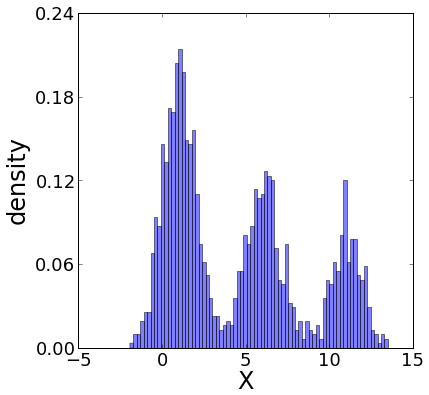
\includegraphics[width=0.7\textwidth, height=0.9\textheight, keepaspectratio]{_fig_01.png}
\par
\end{center}
\end{codeoutput}
\end{codecell}
\begin{codecell}
\begin{codeinput}
\begin{lstlisting}
## Estimate the level set tree - the easy way
tree = gtree.geomTree(X, k, gamma, n_grid=None, verbose=True)
print tree


## Retrieve cluster assignments from the tree
uc, leaves = tree.getClusterLabels(method='all-mode')
print "cluster counts:", np.bincount(uc[:, 1])
print "leaf indices:", leaves


## Plot the level set tree with colored leaves
## note the plot function returns a tuple with 5 objects. The first member of 
## tuple is the figure, which for most users is the only interesting part.
fig = tree.plot(form='lambda', width='uniform', color_nodes=leaves)[0]
fig.show()
\end{lstlisting}
\end{codeinput}
\begin{codeoutput}

\begin{verbatim}
iteration 0
iteration 100
iteration 200
iteration 300
iteration 400
iteration 500
iteration 600
iteration 700
iteration 800
iteration 900
iteration 1000
iteration 1100
iteration 1200
iteration 1300
iteration 1400
       alpha1    alpha2  children   lambda1   lambda2 parent  size
key                                                               
0    0.000000  0.019333    [1, 2]  0.000000  0.015125   None  1500
1    0.019333  0.044667    [3, 4]  0.015125  0.020686      0  1198
2    0.019333  0.442000        []  0.015125  0.090257      0   273
3    0.044667  0.688667  [37, 38]  0.020686  0.156450      1   763
4    0.044667  0.706000        []  0.020686  0.163335      1   417
37   0.688667  0.976667        []  0.156450  0.267754      3   341
38   0.688667  0.958667        []  0.156450  0.252876      3    94
cluster counts: [273 417 341  94]
leaf indices: [2, 4, 37, 38]

\end{verbatim}
\begin{center}
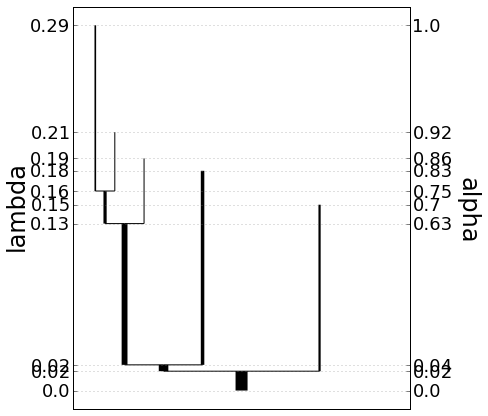
\includegraphics[width=0.7\textwidth, height=0.9\textheight, keepaspectratio]{_fig_03.png}
\par
\end{center}
\end{codeoutput}
\end{codecell}
\begin{codecell}
\begin{codeinput}
\begin{lstlisting}
## Assign background points
fc = utl.assignBackgroundPoints(X.reshape((n, -1)), uc, method='knn', k=9)
print "final cluster counts:", np.bincount(fc[:, 1])
\end{lstlisting}
\end{codeinput}
\begin{codeoutput}

\begin{verbatim}
final cluster counts: [289 455 536 220]

\end{verbatim}

\end{codeoutput}
\end{codecell}
Switch to a 2D example with finer control of the individual components
of tree estimation.

\begin{codecell}
\begin{codeinput}
\begin{lstlisting}
## Add the stats package for kernel density estimation
import scipy.stats as spstat

## Re-set data parameters
n = 1500
p_k = 0.005
p_gamma = 0.01
mix = (0.5, 0.3, 0.2)

k = int(p_k * n)
gamma = int(p_gamma * n)

ctr = ((1, 5), (4, 5), (5, 1))
sdev = (0.5*np.eye(2),) * 3


## Generate data
membership = np.random.multinomial(n, pvals=mix)
p = len(ctr[0])
X = np.zeros((n, p), dtype=np.float)
g = np.zeros((n, ), dtype=np.int)
b = np.cumsum((0,) + tuple(membership))

for i, (size, mu, sigma) in enumerate(zip(membership, ctr, sdev)):
	ix = range(b[i], b[i+1])
	X[ix, :] = np.random.multivariate_normal(mu, sigma, size)
	g[ix] = i


## Scatterplot, to show the simulation worked
fig, ax = plt.subplots()
ax.scatter(X[:,0], X[:,1], s=50, c=g, alpha=0.3)
fig.show()
\end{lstlisting}
\end{codeinput}
\begin{codeoutput}
\begin{center}
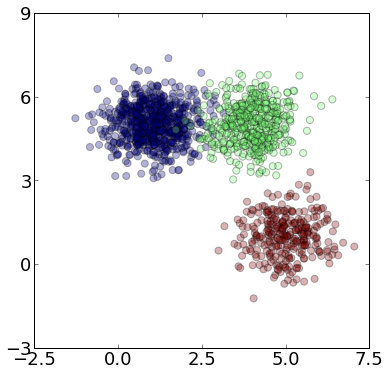
\includegraphics[width=0.7\textwidth, height=0.9\textheight, keepaspectratio]{_fig_05.png}
\par
\end{center}
\end{codeoutput}
\end{codecell}
\begin{codecell}
\begin{codeinput}
\begin{lstlisting}
## Construct the similarity graph and density estimate
W, k_radius = utl.knnGraph(X, k, self_edge=False)
kernel = spstat.gaussian_kde(X.T)
fhat = kernel(X.T)


## Construct the level set tree
bg_sets, levels = utl.constructDensityGrid(fhat, mode='mass', n_grid=300)
tree = gtree.constructTree(W, levels, bg_sets, mode='density', verbose=True)
print tree
\end{lstlisting}
\end{codeinput}
\begin{codeoutput}

\begin{verbatim}
iteration 0
iteration 100
iteration 200
       alpha1    alpha2  children   lambda1   lambda2 parent  size
key                                                               
0    0.000000  0.006667    [1, 2]  0.000000  0.003153   None  1500
1    0.006667  0.387333    [5, 6]  0.003153  0.038202      0  1201
2    0.006667  0.120000    [3, 4]  0.003153  0.017841      0   289
3    0.120000  0.404667    [7, 8]  0.017841  0.039015      2   201
4    0.120000  0.123333        []  0.017841  0.018351      2     1
5    0.387333  0.882667  [11, 12]  0.038202  0.088096      1   589
6    0.387333  0.732000   [9, 10]  0.038202  0.065463      1   314
7    0.404667  0.418000        []  0.039015  0.040040      3     5
8    0.404667  0.408000        []  0.039015  0.039220      3     3
9    0.732000  0.738667        []  0.065463  0.066172      6     2
10   0.732000  0.748667        []  0.065463  0.067523      6    10
11   0.882667  0.922667  [13, 14]  0.088096  0.094461      5   175
12   0.882667  0.896000        []  0.088096  0.090142      5     1
13   0.922667  0.976000  [15, 16]  0.094461  0.101287     11   115
14   0.922667  0.926000        []  0.094461  0.095457     11     1
15   0.976000  1.000000        []  0.101287  0.105238     13    31
16   0.976000  0.979333  [17, 18]  0.101287  0.101752     13     5
17   0.979333  0.989333        []  0.101752  0.103493     16     1
18   0.979333  0.989333        []  0.101752  0.103493     16     2

\end{verbatim}

\end{codeoutput}
\end{codecell}
\begin{codecell}
\begin{codeinput}
\begin{lstlisting}
## Save and/or load a tree (obviously redundant in this tutorial)
tree.save('test_tree')
tree = gtree.loadTree('test_tree')


## Prune the tree
tree.mergeBySize(gamma)
print tree
\end{lstlisting}
\end{codeinput}
\begin{codeoutput}

\begin{verbatim}
       alpha1    alpha2 children   lambda1   lambda2 parent  size
key                                                              
0    0.000000  0.006667   [1, 2]  0.000000  0.003153   None  1500
1    0.006667  0.387333   [5, 6]  0.003153  0.038202      0  1201
2    0.006667  0.418000       []  0.003153  0.040040      0   289
5    0.387333  1.000000       []  0.038202  0.105238      1   589
6    0.387333  0.748667       []  0.038202  0.067523      1   314

\end{verbatim}

\end{codeoutput}
\end{codecell}
\begin{codecell}
\begin{codeinput}
\begin{lstlisting}
## Interactive tools
#tool = gtree.ComponentGUI(tree, X, form='alpha', width='mass', output=['scatter'])
#tool = gtree.ClusterGUI(tree, X, form='alpha', width='mass', output=['scatter'])
#tool.show()
\end{lstlisting}
\end{codeinput}

\end{codecell}
\begin{codecell}
\begin{codeinput}
\begin{lstlisting}
## Get foreground clusters and plot them
uc, nodes = tree.getClusterLabels(method='first-k', k=3)

fig, ax = utl.plotForeground(X, uc, s=50, alpha=0.5)
fig.show()
\end{lstlisting}
\end{codeinput}
\begin{codeoutput}
\begin{center}
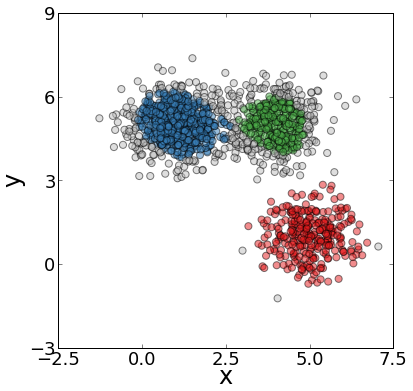
\includegraphics[width=0.7\textwidth, height=0.9\textheight, keepaspectratio]{_fig_08.png}
\par
\end{center}
\end{codeoutput}
\end{codecell}
\begin{codecell}
\begin{codeinput}
\begin{lstlisting}
## Plot the basic lambda scale tree
fig = tree.plot(form='lambda', width='uniform', color_nodes=nodes)[0]
fig.show()
\end{lstlisting}
\end{codeinput}
\begin{codeoutput}
\begin{center}
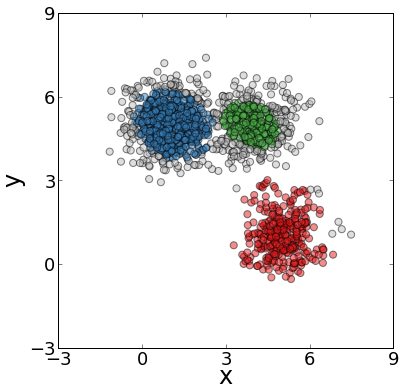
\includegraphics[width=0.7\textwidth, height=0.9\textheight, keepaspectratio]{_fig_09.png}
\par
\end{center}
\end{codeoutput}
\end{codecell}
\begin{codecell}
\begin{codeinput}
\begin{lstlisting}
## Plot the basic level set tree with mass-based spacing
fig = tree.plot(form='lambda', width='mass', color_nodes=nodes)[0]
fig.show()
\end{lstlisting}
\end{codeinput}
\begin{codeoutput}
\begin{center}
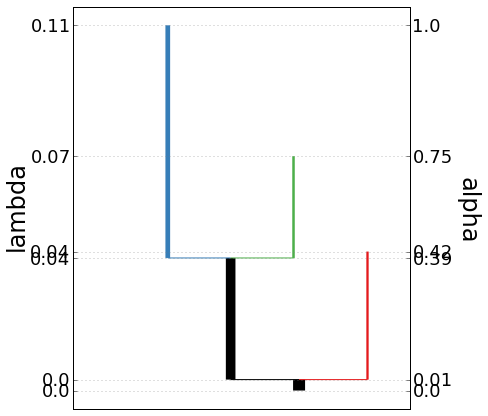
\includegraphics[width=0.7\textwidth, height=0.9\textheight, keepaspectratio]{_fig_10.png}
\par
\end{center}
\end{codeoutput}
\end{codecell}
\begin{codecell}
\begin{codeinput}
\begin{lstlisting}
## Plot the level set tree with alpha scale
fig = tree.plot(form='alpha', width='mass', color_nodes=nodes)[0]
fig.show()
\end{lstlisting}
\end{codeinput}
\begin{codeoutput}
\begin{center}
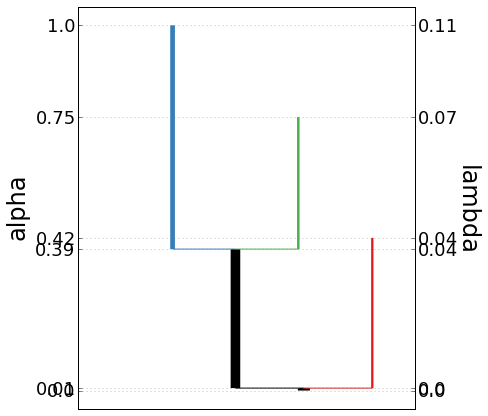
\includegraphics[width=0.7\textwidth, height=0.9\textheight, keepaspectratio]{_fig_11.png}
\par
\end{center}
\end{codeoutput}
\end{codecell}
\begin{codecell}
\begin{codeinput}
\begin{lstlisting}
## Plot the level set tree with kappa scale
fig = tree.plot(form='kappa', width='mass', color_nodes=nodes)[0]
fig.show()
\end{lstlisting}
\end{codeinput}
\begin{codeoutput}
\begin{center}
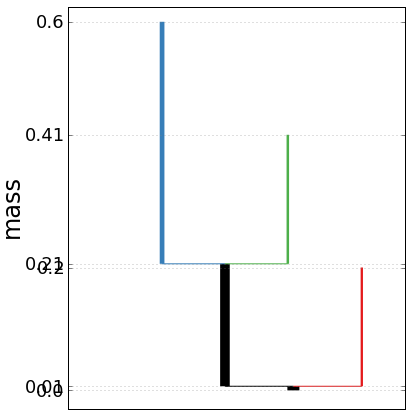
\includegraphics[width=0.7\textwidth, height=0.9\textheight, keepaspectratio]{_fig_12.png}
\par
\end{center}
\end{codeoutput}
\end{codecell}
\begin{codecell}
\begin{codeinput}
\begin{lstlisting}

\end{lstlisting}
\end{codeinput}

\end{codecell}



\end{document}

